\documentclass[conference]{IEEEtran}
\usepackage{url}
\hyphenation{op-tical net-works semi-conduc-tor}
\usepackage{graphicx}

\begin{document}
\title{From Python to Pythonic}


\author{
\IEEEauthorblockN{José Javier Merchante}
\IEEEauthorblockA{
Universidad Rey Juan Carlos\\
Fuenlabrada, Madrid, Spain\\
Email: jj.merchante@gmail.com}
\and
\IEEEauthorblockN{Gregorio Robles}
\IEEEauthorblockA{GSyC/LibreSoft\\
Universidad Rey Juan Carlos\\
Fuenlabrada, Madrid, Spain\\
Email: grex@gsyc.urjc.es}
}


\maketitle
\IEEEpeerreviewmaketitle

\section{Introduction}

Every programming language has its culture and usual way to code a task in a specific language, that's what programmers usually call idioms. For an advanced programmer there is always one way of accomplishing one task that perform the readability instead of writing the implementation it replaces from another language.

Python is a programming language that in the last years has grown a lot. For this language there are many tools that checks the code against some style conventions written in PEP8, but there aren't any popular tool that identify what idioms you are using and which one could help you to improve your code, and exists a large Python community that is concerned in writing Python the right way and are actively providing ideas.

Many Python books and web pages explain the language without including this idioms, and focus on explain the language like it was another language but with Python syntax, falling in mistakes like:

\begin{verbatim}
colors = ["blue", "red", "yellow"]

for i in range(len(colors)):
    print colors[i]
\end{verbatim}

It is inadvisable and the learner must to know that there is right way to do that:

\begin{verbatim}
colors = ["blue", "red", "yellow"]

for color in colors:
    print color
\end{verbatim}

For this reasons, it is necessary a tool that store all this idioms, and help beginners and advanced programmers to code more legible, readable and write the task the right way. That is what the Python community call "Pythonic".

\section{Methodology}

The implementation of this software was carried out with the search of the most important Python idioms in advanced books and conferences of people that is very interested in writing pythonic code. By this way, it has been done a deep leaning of more that 100 Python idioms with distinctive difficult levels. A list of some Python idioms is as follows:

\begin{itemize}
\item Comprehensions
\item Magic methods
\item Lambda functions
\item Decorators
\item Collections structures
\item Class methods
\item Closures
\item ...
\end{itemize}

The research methodology was based on mining GitHub, downloading those repositories which main language is Python. We found more than 700.000 but only got 70.000 for lack of space and because it was a good sample to get statistics.

From those downloaded repositories, we could obtain a lot of data like idioms, anti-idioms, and also the authors of each one.

In order to identify the idioms, we use a lexer called Pygments to make each idiom a sequence of tokens that later we should find in the Python code.

For each idioms found, we also get the author from the output of \texttt{git blame}. That allow to obtain the pythonic contribution of each collaborator to one GitHub project and in this way make statistics.

The analysis of the repositories took weeks, there were about 500 GB of them (previously deleted no Python files in order to get more storage). The Python idioms found were stored in a database locally. Those results were analyzed with Pandas software to get some graphics that answer some questions like: What are the idioms mostly used? Which are the less one? Are there richer repositories in idioms that others? What is the mean of idioms per repository?

\section{Results}

The identification of the idioms and the subsequent analysis was successful. We could obtain some statistics that answer some of the questions previously performed and much more.

For example, in figure 1 display the most used idioms in each repository. This figure shows the idioms that are at least 1 time in each repository. As we can see, decorators and list comprehensions, are two of the most common Python idioms. The sentence \verb|if __name__ == "__main__"| is also at least one time in each repository.

The two first are other special idioms that maybe they shouldn't be considered because the number of appearance of them. The first one is the function call that is made with the equal operator and the second one is just to check how many repositories are documented.

\begin{figure}[ht]
\centering
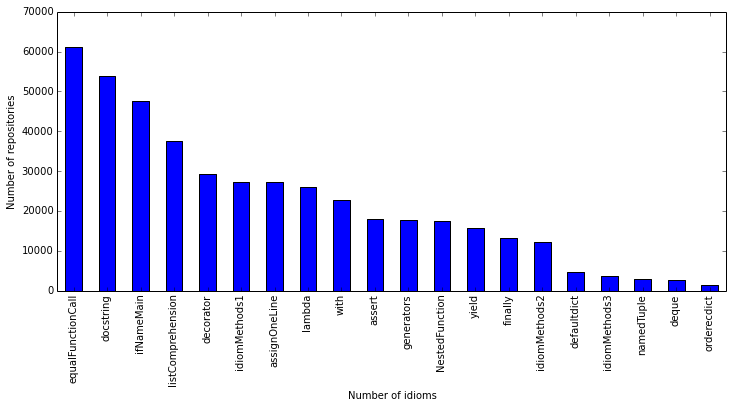
\includegraphics[width=80mm]{img/num_idiom_repo.png}
\label{fig:idiom_ranking}
\caption{Pythonic idioms ranking}
\end{figure}

Others of the most used idioms, but are grouped in order of complexity, are the magic methods (methods that are invoked when you use certain syntax). In figure 2 we can see the number of occurrences of each of them without been grouped. 

\begin{figure}[ht]
\centering
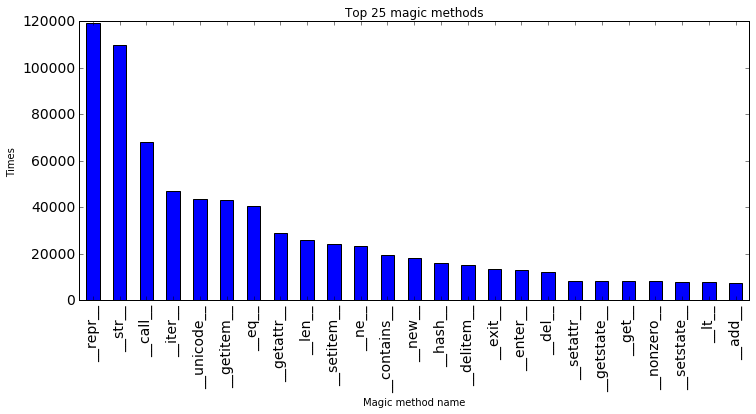
\includegraphics[width=80mm]{img/magic_methods.png}
\label{fig:magic_ranking}
\caption{Magic methods most common}
\end{figure}

One of the most usual is \verb|__init__|, but is omitted due to is necessary for creating a class and couldn't be consider a Python idiom.

The last figure shows the number of idioms in each repository. This curve show that many of the repository have few idioms, but actually more than 50\% have more than 40 idioms and the mean is 304.52

\begin{figure}[ht]
\centering
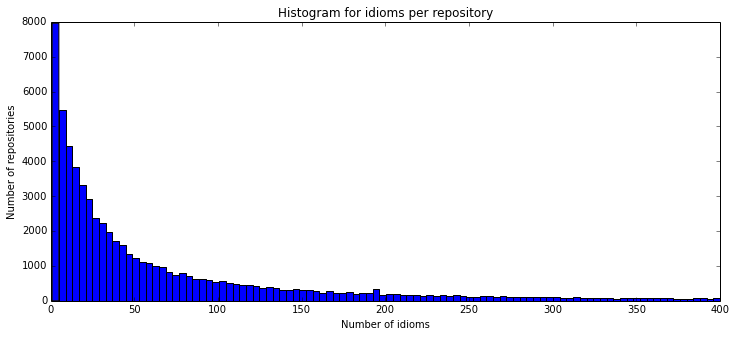
\includegraphics[width=80mm]{img/idioms_per_repository.png}
\label{fig:idioms_per_repository}
\caption{Number of idioms per repository}
\end{figure}

\end{document}

